% com-cas-poster
% by hk, rj, June 2012

\documentclass[final]{beamer} 

\mode<presentation> {  
    %\usetheme{Warsaw}
    \usetheme{Boadilla}
    %\usetheme{Montpellier}
    %\usetheme{Singapore}
    %\usetheme{Ilmenau}
    %\usetheme{Berkeley}
    %\usetheme{Madrid}
}

\usepackage[english]{babel}
%hk% \usepackage[latin1]{inputenc}
\usepackage{relsize}
\usepackage{listings}

\usepackage{epsfig}

\usepackage{amssymb}
%\usepackage{amsmath,amsthm, amssymb, latexsym}
\usefonttheme[onlymath]{serif}
\boldmath

\usepackage[orientation=landscape,size=a1,scale=1.4]{beamerposter}

\newcommand{\code}[1]{\texttt{#1}}


\title[Categories and Mixins]{Categories as classes and mixin composition}

\author[Kredel \& Jolly]{Heinz Kredel\inst{1} and Raphael Jolly\inst{2}} 

\institute{IT-Center, University of Mannheim, Germany %,
%\email{kredel@rz.uni-mannheim.de,}
\and Databeans, Paris, France%,
%\email{raphael.jolly@free.fr}
}

%\date{Jun. 7th, 2012}


\begin{document}

  %hk: makes new page% \maketitle

\begin{frame}[fragile] 
\frametitle{\hspace{13cm}Categories as classes and mixin composition, Heinz Kredel and Raphael Jolly}
%\hfill
\begin{columns}[t]

\begin{column}{.3\linewidth}

  \begin{block}{\large Contents}
  \normalsize 
  \begin{enumerate}
  \item generic, strongly typed, object oriented computer algebra software
  \item concept of categories 
  \item software, algorithm implementations can be packaged and
    re-combined using traits in a category-like fashion
  \end{enumerate}
  \end{block}
  \hfill
  \begin{block}{\large Introduction}
{\scriptsize
The modeling of algebraic structures in a strongly typed, generic,
object oriented computer algebra software has been presented with the
systems JAS and ScAS.
The design and implementation of these strongly typed, generic and
object oriented polynomial algorithm libraries in Java and Scala is
presented in papers.  
The libraries are enhanced for interactive usage with the help of the Jython and
JRuby scripting languages. The libraries now
provide several algorithm versions for greatest common divisor,
squarefree decomposition, factorization and Gr\"obner bases
computation in separate packages.
\par}\par
  \end{block}
  \hfill
  \begin{block}{\large Related Work}
\scriptsize
Magma [BosmaCannonPlayoust:1997], Sage [Stein:2005], 
Axiom [JenksSutor:1992,Watt:2003]
\par
{\scriptsize Acknowledgments}\par
{\tiny Thomas Becker, Wolfgang K. Seiler, Thomas Sturm, Axel Kramer, 
Jaime Gutierrez, Sherm Ostrowsky, Markus Aleksy\par}
  \end{block}
  \hfill
  \begin{block}{\large Categories in CAS}
  \scriptsize
  \begin{enumerate}
  \item Axiom, Aldor: abstract classes
  \item Magma, Sage: classes with same representation
  \end{enumerate}
  \end{block}
  \hfill
  \begin{block}{\large Generic, strongly typed, object oriented computer algebra software}
      \centering
      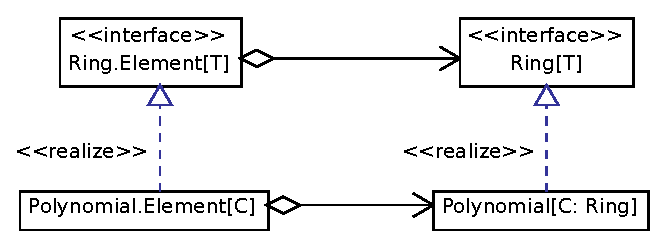
\epsfig{file=BasicTypes,clip=,width=0.85\linewidth}
  \end{block}
  \hfill
\end{column}


\begin{column}{.3\linewidth}
 
  \begin{block}{\large Example}
%\footnotesize \scriptsize %
\tiny 
%code example in ScAS syntax - maybe we need to translate
%the uml diagram as well ?
\begin{lstlisting} 
 import Implicits.QQ
 implicit val r = Polynomial(QQ, "w")
 val Array(w) = r.generators
 val a = pow(w, 2) - 2 
\end{lstlisting} 
%\begin{verbatim} 
%BigRational rf = new BigRational(1); 
%GenPolynomialRing<BigRational> pf 
% = new GenPolynomialRing<BigRational>(rf,new String[]{"w"});
%GenPolynomial<BigRational> a = pf.parse("w^2 - 2");
%\end{verbatim}
  \end{block}
  \hfill
  \begin{block}{\large Algorithm libraries}
  \scriptsize 
  \begin{itemize}
  \item focus on multivariate polynomials
  \item greatest common divisor: \code{gcd()}, \code{content()}
  \item squarefree decomposition: finite or infinite fields of characteristic 0 or $p$
  \item factorization: depends on the explicit coefficient ring
  \end{itemize}
  \end{block}
  \hfill
  \begin{block}{\large Code Organization Problem}
  \scriptsize 
The algebraic structures and elements of them together
with the algorithm libraries provide a precise way to use a suitable
combination for a given situation. It is, however, elaborate and one
would like to combine or package together certain configurations to be
able to deploy and use them as a single object or thing. 
  \end{block}
  \hfill
  \begin{block}{\large Mixins for category-like software organization}
{\scriptsize %\footnotesize 
We seek to apply modern computer language ability for reusable
component design and implementation to the case of computer algebra
software. We need to create components for each algorithm flavor
(for GCD computation : different polynomial remainder sequences,
modular : Chinese remainder or Hensel) and to tie them together
in a single object. This requires some kind of multiple inheritance,
which is not available in Java, but is in recent programming
languages like Scala, in the form of {\em mixins}, or traits.
\par}\par
  \end{block}
\hfill
\end{column}


\begin{column}{.3\linewidth}

  \begin{block}{\large Preliminary definitions}
\tiny %\scriptsize
\begin{lstlisting}
 trait Ring[T] {
   def plus(x: T, y: T): T
 }
 import Polynomial.Element
 trait Polynomial[C: Ring] extends Ring[Element[C]] {
   def plus(x: Element[C], y: Element[C]) = ...
 }
 object Polynomial {
   trait Element[C: Ring]
 }
\end{lstlisting}
  \end{block}
  \hfill
  \begin{block}{\large Peer (mixin) vs hierarchical composition}
\tiny %\scriptsize
{\footnotesize In hierarchical composition, work is delegated to
a member ring:}\par
\begin{lstlisting}
 trait GCDEngine[C: Ring] {
   val ring: Polynomial[C]
   def gcd(x: Element[C], y: Element[C]): Element[C]
 }
 trait GCDSimple[C: Ring] extends GCDEngine[C] {
   def gcd(x: Element[C], y: Element[C])=// use ring.plus etc.
 }
 val e = new GCDSimple[BigInteger] {
   val ring = new Polynomial[BigInteger]
 }
\end{lstlisting}
{\footnotesize The same effect can be obtained through a mixin:}\par
\begin{lstlisting}
 trait GCDSimple[C: Ring] extends Polynomial[C] {
   def gcd(x: Element[C], y: Element[C])=// use this.plus etc.
 }
 val r = new Polynomial[BigInteger] with GCDSimple[BigInteger]
\end{lstlisting}
  \end{block}
  \hfill
  \begin{block}{\large Classes, mixin composition and categories}
\tiny %\scriptsize
{\footnotesize We can combine several algorithms:}\par
\begin{lstlisting}
trait GCDEngineX[C: Ring] extends Polynomial[C] {
  def gcd(x: Element[C], y: Element[C]) = ...
}
trait SquarefreeEngineY[C: Ring] extends Polynomial[C] {
  def squarefreePart(x: Element[C]): Element[C] = ...
  def squarefreeFactors(x: Element[C]): List[Element[C]]=...
}
trait FactorEngineZ[C: Ring] extends Polynomial[C] {
  def factorList(x: Element[C]): List[Element[C]] = ...
  def factors(x: Element[C]): Map[Element[C], Long] = ...
}
val r = new Polynomial[BigRational]
        with GcdEngineX[BigRational] 
        with SquarefreeEngineY[BigRational]
        with FactorEngineZ[BigRational]
\end{lstlisting}
{\footnotesize Some algorithms may need further specialization
of the coefficient type:}\par
\begin{lstlisting}
trait GCDModular extends Polynomial[BigInteger] {
  def gcd(x: Element[BigInteger], y: Element[BigInteger])=...
}
val r = new Polynomial[BigInteger] with GCDModular
\end{lstlisting}
{\footnotesize The desired packaging can be pre-setup or chosen
automatically according to the coefficient type:}\par
\begin{lstlisting}
val r = Polynomial(ring, pp) // might return an object
(category) of type GCDModular if ring is BigInteger and so on
\end{lstlisting}
  \end{block}
  \hfill
\end{column}

\end{columns}

%\vfill
\end{frame}

%\begin{frame}[fragile] 
%\frametitle{Next page}
%\vfill
%\begin{columns}[t]
%\begin{column}{.3\linewidth}
%  \hfill
%\end{column}
%
%\begin{column}{.3\linewidth}
%  \begin{block}{\large References}
%\footnotesize
%\bibliographystyle{splncs}
%\bibliography{com-cas}
%  \end{block}
%\end{column}
%
%\end{columns}
%
%\vfill
%\end{frame}

\end{document}
